\chapter{JDBC}
\label{chap:jdbc}

\fcolorbox{black}[HTML]{E9F0E9}{\parbox{\textwidth}{%
\noindent \textbf{Learning goals}\\
The junior-colleague
\begin{enumerate}[nolistsep]
\item can describe what JDBC is.
\item can explain the benefits of JPA over JDBC.
\item can identify the base interfaces of JDBC.
\item can use JDBC to connect to a database.
\item can use JDBC to query a database.
\item can use JDBC to create a table.
\item can use JDBC to insert, update, and delete records in a table.
\item can use transactions in a JDBC application.
\item can describe what SQL injection is.
\item can use Prepared Statements to prevent SQL injection.
\item can explain the ACID-properties of a transaction.
\item can explain different isolation levels and the problems that can possibly occur.
\item can describe and implement the Data Access Object Pattern.
\end{enumerate}}}

TODO REVIEW https://www.marcobehler.com/guides/jdbc

\fcolorbox{black}[HTML]{ADD8E6}{\parbox{\textwidth}{%
\noindent \textbf{Source for this chapter:}\\
SampleJPAProject: \url{https://github.com/custersnele/SampleJPAProject}
This project uses the mysql music database used in chapter \ref{chap:jdbc}. 
}}

\section{Why not JDBC?}

JDBC is a low-level API. When using JDBC you have to write quite some boilerplate code.
Take for example the code for mapping the data from the ResultSet to your actual objects.

\begin{lstlisting}[frame=single, language=java]
List<User> users = new ArrayList<User>();
while(rs.next()) {
     User user = new User();
     user.setId(rs.getString("userid"));
     user.setName(rs.getString("firstname"));
     user.setEmail(rs.getString("email"));
     users.add(user);
 }
 \end{lstlisting}

With JDBC, your SQL statement interwine with your Java code,  which makes your code  hard to refactor and your datasources or DAOs might end up messy (e.g.  MusicDatasource).

\section{What is JDBC?}

JDBC or Java Database Connectivity is Java's low-level API for making database connections and handling SQL queries and responses.

JDBC is an adapter layer from Java to SQL. It gives Java developers a common interface for connecting to a database, issuing queries and commands, and managing responses.


\section{The database}

We will be using docker to supply the database in our development environment.  In case anything goes wrong, you simply recreate your environment from scratch. 
There are some advantages of using docker on your development machine:
There’s less clutter on your  machine and you can easily work on multiple projects with different database versions. 

For this chapter you need a mysql database with a music database. The database has tables for albums, songs and artists. The script for creating the docker container with the music\_db can be found in the folder src/main/docker of the demo project which is available on github:


\section{JDBC Interfaces}

\begin{lstlisting}[language=java,frame=single]
import java.sql.Connection;
import java.sql.DriverManager;
import java.sql.SQLException;
import java.sql.ResultSet;
import java.sql.Statement;
\end{lstlisting}

Each of these imports provides access to a class that facilitates the standard Java database connection:
Connection represents the connection to the database.
DriverManager obtains the connection to the database. (Another option is DataSource, used for connection pooling. )
ResultSet and Statement model the data result sets and SQL statements.
SQLException handles SQL errors between the Java application and the database.


\begin{figure}[t]
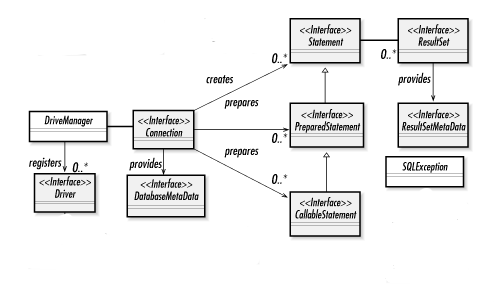
\includegraphics[width=\textwidth]{./images/chapter4/jdbc_diagram.png}
\centering
\end{figure}

\section{Slides}

% \includepdf[
%    pages=-,
%    frame,
%    pagecommand={}]{chapter_jdbc_slides.pdf}